%(BEGIN_QUESTION)
% Copyright 2006, Tony R. Kuphaldt, released under the Creative Commons Attribution License (v 1.0)
% This means you may do almost anything with this work of mine, so long as you give me proper credit

En enkel måte å bygge referanseskjøtkompensasjon på, er å bruke en bro med termistor (temperaturfølsom motstand) i én arm:

$$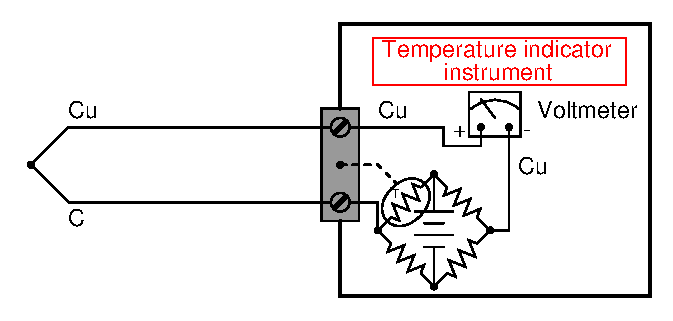
\includegraphics[width=15.5cm]{i00384x01.eps}$$

Når terminalblokken varmes opp eller kjøles ned, endres termistormotstanden. Da endres brobalansen og legger på riktig spenningsbidrag i serie med målekretsen, slik at millivoltspenningen fra termoelementledningene mot kobberledningene i terminalblokken (``referanseskjøten'') kanselleres.

Gitt termoelementtype vist her (type T med kobber og constantan), voltmeterpolaritet, batteriorientering i broen og termistorens plassering i broen: Må termistoren ha {\it positiv} temperaturkoeffisient (motstand øker når temperatur øker), eller {\it negativ} temperaturkoeffisient (motstand minker når temperatur øker)?

Hint: Start med å identifisere selve feilkilden -- bestem polariteten til referanseskjøtspenningen, slik at du vet hvilken polaritet brospenningen må ha for å kansellere den.

\vskip 20pt \vbox{\hrule \hbox{\strut \vrule{} {\bf Forslag til sokratisk diskusjon} \vrule} \hrule}

\begin{itemize}
\item{} Hvilken type temperaturkoeffisient har en RTD?
\item{} Anta at termistoren ikke har riktig {\it størrelse} på temperaturkoeffisienten (feil ``alpha''). Påvirkes systemets {\it nullpunkt}, {\it span}, eller begge?
\item{} Hvis vi må bruke termistor for referanseskjøtkompensasjon i et termoelement, hvorfor bruker vi da termoelement i prosessen i det hele tatt? Hvorfor ikke bare bruke termistor i prosessen?
\item{} Hvis termistoren feiler med brudd: går voltmeteret opp eller ned på skala?
\item{} Hvis termistoren feiler kortsluttet: går voltmeteret opp eller ned på skala?
\end{itemize}

\underbar{file i00384}
%(END_QUESTION)





%(BEGIN_ANSWER)

Først bestemmer vi polariteten på referanseskjøtspenningen ved nedre terminal, der constantan (C) møter kobber (Cu). Siden kobber er positiv leder i kobber-constantan-skjøt, blir polariteten positiv på høyre side og negativ på venstre side. Dette vises i figuren både med +/- og med piler (pilspiss er positiv):

$$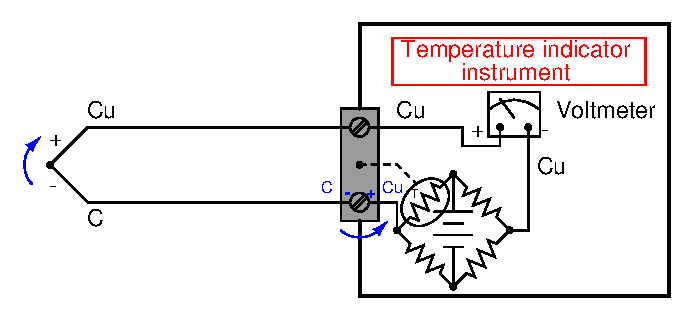
\includegraphics[width=15.5cm]{i00384x02.eps}$$

For å motvirke denne millivoltspenningen må brospenningen være positiv til venstre og negativ til høyre:

$$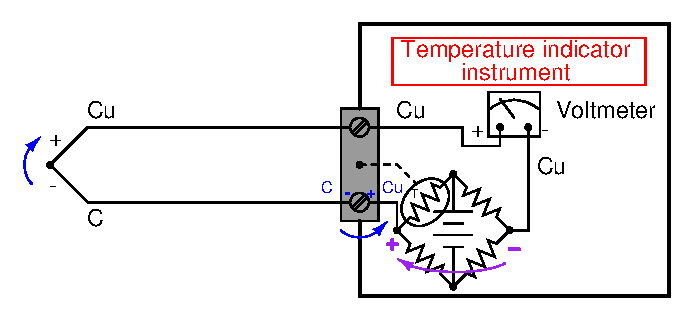
\includegraphics[width=15.5cm]{i00384x03.eps}$$

Jo varmere referanseskjøten blir, jo større spenning gir den. Broen må derfor også gi større motspenning når termistortemperaturen øker. For at venstre broterminal skal bli mer positiv (og høyre mer negativ), gitt batteri med positiv ``opp'' og negativ ``ned'', må termistorverdien {\it minke}. Dermed trenger vi en termistor med {\bf negativ temperaturkoeffisient}.

\vskip 10pt

Termoelementer er fortsatt verdifulle som primærsensorer fordi de har langt større temperaturområde enn termistorer, og de er ofte mer robuste.


%(END_ANSWER)





%(BEGIN_NOTES)


%INDEX% Measurement, temperature: thermocouple

%(END_NOTES)
